\chapter{Results \& Discussion} % Main chapter title

\label{Chapter5} % Change X to a consecutive number; for referencing this chapter elsewhere, use \ref{ChapterX}

In Chapter \ref{Chapter3} we established the source and details of the Amazon product review dataset and Chapter \ref{Chapter4} addressed the details of the models and techniques adopted in our analysis of building several recommender systems.  This has provided a platform for which we can critically address the primary research questions for this thesis, raised in Section \ref{sec:1 Research Questions and Significance}, by evaluating the various recommender system's predictive accuracy and top-$n$ capability. 

Specifically, this chapter will present the results of the experiments conducted to evaluate the performance of the models described in Chapter \ref{Chapter4}. The results will be presented in the context of the research questions and the previous literature within this domain. We first look at the results of the experiments in Section \ref{sec:5 Results}. Section \ref{sec:5 Discussion} explores the results of the models in the context of the research questions and the previous literature within this domain. The chapter concludes by providing a summary of the results and discussion, in Section \ref{sec:5 Conclusion for Results}.


\section{Results}
\label{sec:5 Results}

In this section we display the results from our analysis, comparing the performance of several different recommenders under two different tasks - rating prediction (Section \ref{subsec:Predictive Accuracy Results}) and top-$n$ evaluation (Section \ref{subsec:5 Top-N Results}). As discussed in Chapter \ref{Chapter4}, the models used in our analysis include the two neighbourhood-based collaborative based approaches (UBCF and IBCF), a model-based collaborative approach (NMF) and the relatively new deep-learning based approach to collaborative filtering (NCF). We built these models for ratings prediction - however, as highlighted in Section \ref{subsec:4 Evaluation Approach}, we evaluated our models under both predictive accuracy and top-$n$ paradigms. 

\subsection{Predictive Accuracy Results}
\label{subsec:Predictive Accuracy Results}

Predictive accuracy, in the context of a recommender system, refers to how well a model is able to predict user preferences or ratings for items \cite{breese2013empirical}. It is usually measured by comparing the predicted ratings to the actual ratings in a dataset. For each user-item pair in the test set, the model makes a prediction about the rating the user would give to the item. The predicted ratings are then compared to the actual ratings in the test set. The measure of how well the model's predictions match the actual ratings is called predictive accuracy \cite{huang2004applying}. The metrics of choice are discussed in detail in Section \ref{sec:2 Evaluation Methods}. Table \ref{tab:pred_acc_res} illustrates the results of our various recommender models. As discussed in Section \ref{sec:4 Modelling Approach}, the NCF model was tested under three different scenarios: using ratings only, using ratings and reviews, and using ratings, reviews, and sentiments. Again, we only include reviews and sentiments in our NCF model - not any of the benchmark models.

\begin{table}[htbp]
    \centering
    \begin{tabular}{|l|l|l|l|l|l|}
    \hline
    \textbf{} & \textbf{Recommender Model} & \textbf{Data Used} & \textbf{MAE} & \textbf{MSE} & \textbf{RMSE} \\
    \hline
    1 &Item-Based Collaborative Filtering & Ratings Only & 0.581 & 0.830 & 0.911 \\
    2 & User-Based Collaborative Filtering & Ratings Only & 0.59 & 0.984 & 0.992 \\
    3& Non-Negative Matrix Factorisation & Ratings Only & 1.583 & 3.467 & 1.862 \\
    4&Neural Collaborative Filtering & Ratings Only & 0.572 & 0.815 & 0.903 \\
    5&Neural Collaborative Filtering & Ratings \& Reviews & \textbf{0.490} & \textbf{0.591} & \textbf{0.769}  \\
    6&Neural Collaborative Filtering & Ratings, Reviews, Sentiments & 0.492 & 0.607 & 0.779 \\
    7&Baseline Model & Ratings Only & 0.67 & 1.270 & 1.311 \\
    \hline
    \end{tabular}
    \caption{Predictive Accuracy Results for Recommender Models Built.}
    \label{tab:pred_acc_res}
\end{table}

The baseline model in Table \ref{tab:pred_acc_res} is a simple model that predicts the average rating for all items. Among these models shown in Table \ref{tab:pred_acc_res}, the NCF model, trained with ratings and reviews (model 5) delivered the most accurate predictions, with an MAE of 0.490, an MSE of 0.591, and an RMSE of 0.769. On the contrary, the NMF model trained with ratings only exhibited the poorest accuracy, recording an MAE of 1.583, an MSE of 3.467, and an RMSE of 1.862. We also noted during our analysis, that both neighbourhood-based approaches, IBCF and UBCF, yielded comparable results. This similarity might be attributed to their shared reliance on the user-item interaction matrix \cite{jia2015user}. 

To determine if the differences in performance between the models are statistically significant, we conducted a paired t-test. This statistical test evaluates whether the differences in the means of two groups are significant or if they could have occurred by random chance \cite{manfei2017differences}. There are a several assumptions that need to be met for the t-test to be valid, including the normality of the data, the homogeneity of variances, the independence of observations and random sampling \cite{manfei2017differences}. For this analysis, we checked whether the assumptions were met and found that they were. Specifically, we found that the data within each group (referring to each recommendation model being evaluated) should follow a normal distribution - the Shapiro-Wilk test\footnote{The Shapiro-Wilk test assesses the normality of data. A p-value greater than the chosen significance level (e.g., 0.05) indicates that the data can be assumed to be normally distributed.} was used to confirm this. We also checked for homogeneity of variances between the groups (referring to the different recommendation models) using Levene's test\footnote{Levene's test evaluates the homogeneity of variances between groups. A non-significant p-value suggests that the variances are approximately equal across groups, which is a prerequisite for t-tests.}. Independence was met since we established consistent data partitioning for each model - so each model was trained and tested on the same data. Lastly, the data was randomly sampled using data partitioning (see Section \ref{sec:3 Data Partitioning}). Thus, we were able to confirm whether the performance differences between NCF with reviews and other models (IBCF, UBCF, and NMF) were statistically significant. The results of the t-test indicated a significant difference in the performance of NCF with reviews (model 5) compared to IBCF ($p$ < 0.01), UBCF ($p$ < 0.01), and NMF ($p$ < 0.01). This confirmed our initial findings that NCF with reviews outperformed other models and that these differences were not due to random chance. 

From Figures \ref{fig:user review distribution} and \ref{fig:product review distribution} in Section \ref{sec:3 Trends and Patterns}, we identified that a key feature of the data is that most products have relatively few reviews (<$50$) and most users have reviewed only a few things (<$20$). This may have implications for the accuracy of the models. For example, the recommender models may be better at predicting ratings for products with more reviews, as it can learn more about the product from the reviews. Similarly, the models may be better at predicting ratings for users with more reviews, as it can learn more about the user from the reviews. To explore this, we can look into the overall accuracy results to see if accuracy depends on any factors - for example, is accuracy higher for users or products with more reviews, or for users with longer review text?

We first look at the impact of the number of reviews per user or item to see if there is a difference in the accuracy of the models for users or items with more reviews. To achieve this, we took users and items in the test set, and assigned them into four groups based on the number of reviews they had. We created these groups by dividing the users and items into quartiles based on the number of reviews they had. We then calculated the average MAE, MSE and RMSE for each group. We can then compare these results to see if the number of reviews has any impact on the accuracy of predictions for users or items who have more reviews. Figures \ref{fig:RMSE_USER_ACC} and \ref{fig:RMSE_ITEM_ACC} show the MSE, RMSE and MAE against the number of reviews for users and items respectively. 

\begin{figure}[htbp]
    \centering
    \begin{subfigure}{0.49\textwidth}
        \centering
        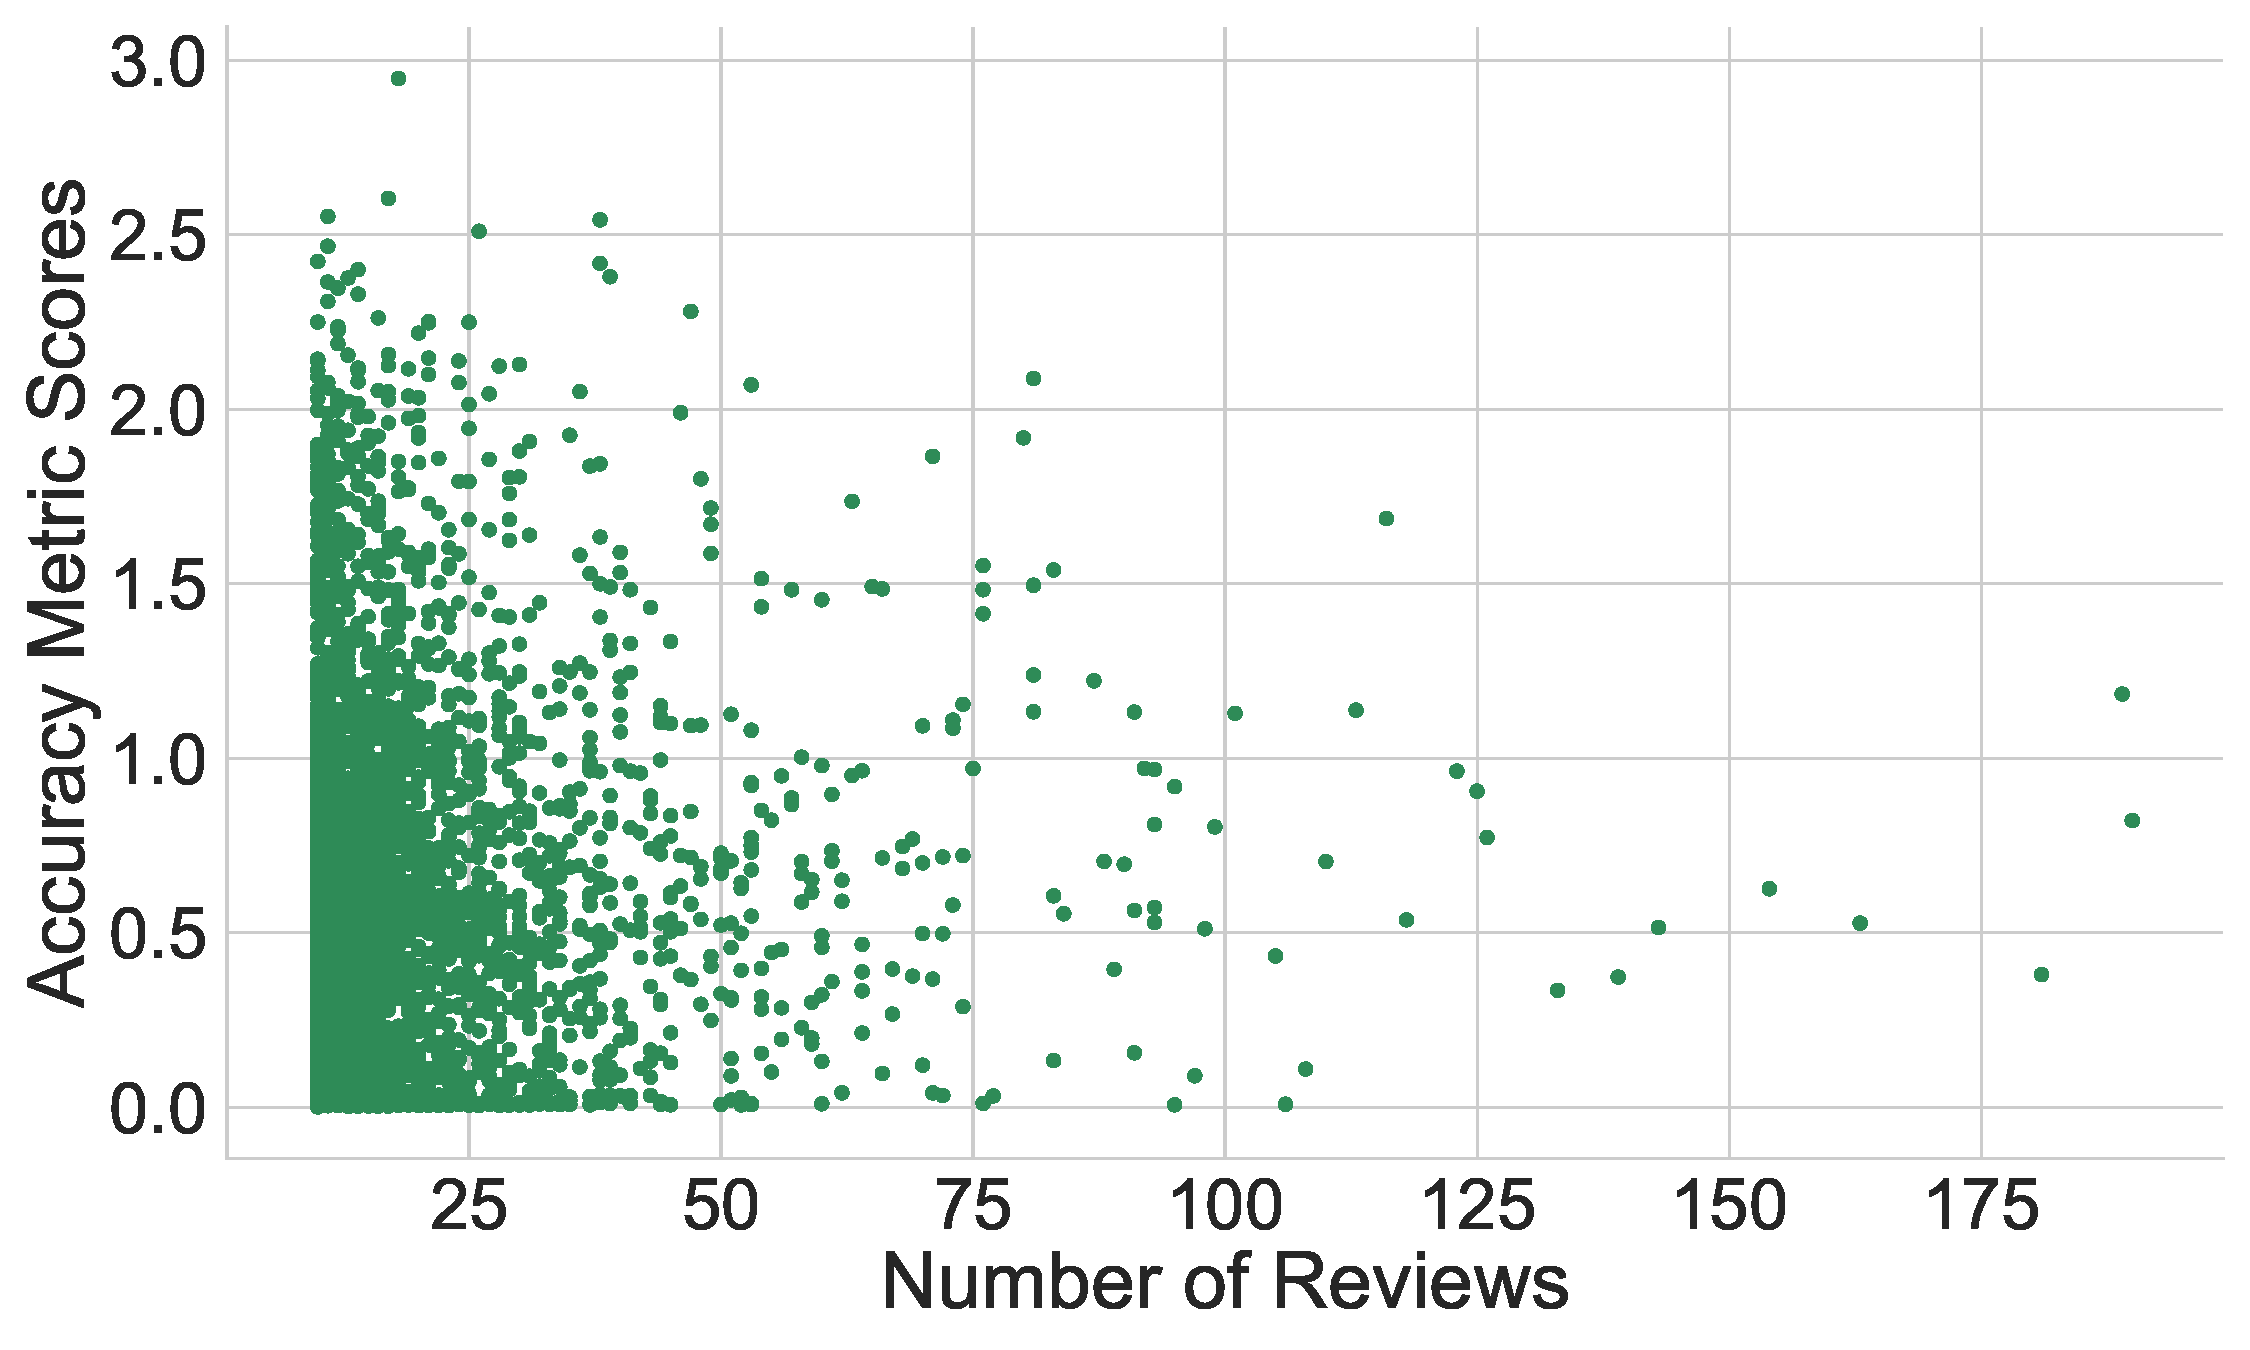
\includegraphics[width=\textwidth]{Figures/ncf_user_ratings_metrics.pdf}
        \caption{Accuracy against the number of reviews for users.}
        \label{fig:RMSE_USER_ACC}
    \end{subfigure}%
    \hfill
    \begin{subfigure}{0.49\textwidth}
        \centering
        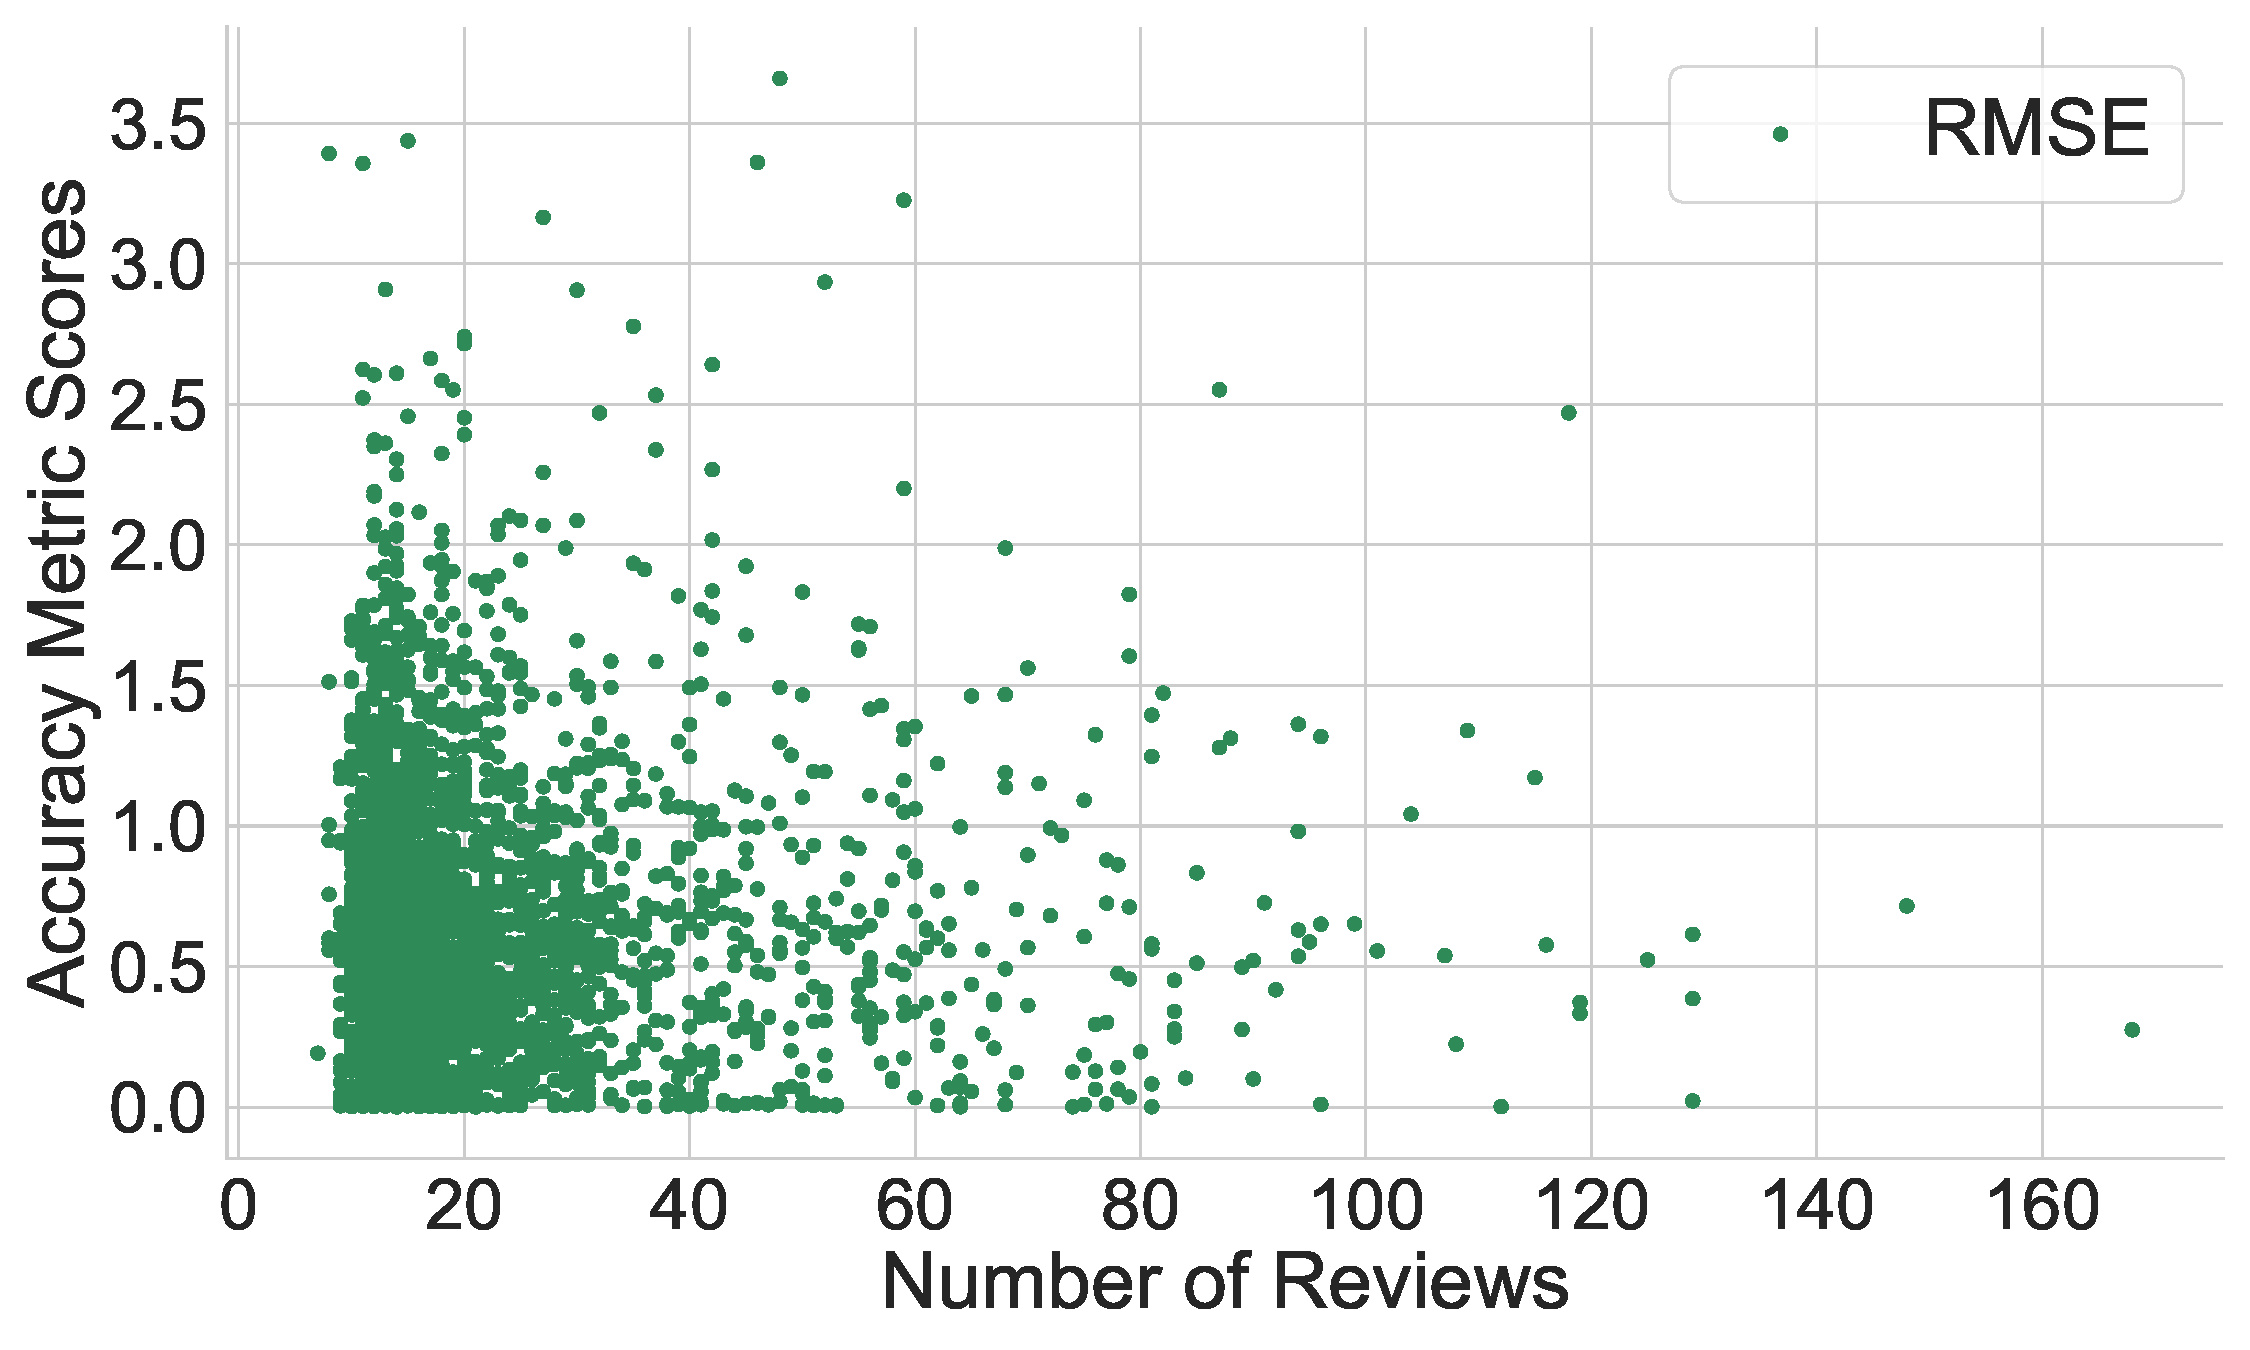
\includegraphics[width=\textwidth]{Figures/ncf_item_ratings_metrics.pdf}
        \caption{Accuracy against the number of reviews for items.}
        \label{fig:RMSE_ITEM_ACC}
    \end{subfigure}
    \caption{Comparison of RMSE for user and item ratings.}
    \label{fig:RMSE_ACC}
\end{figure}


From Figures \ref{fig:RMSE_USER_ACC} and \ref{fig:RMSE_ITEM_ACC}, we can see that the for users and items, those with lower review counts appear to have a wide spread in accuracy (for RMSE). The resulting plots for MSE and MAE show similar results. Those users and items which have higher number of reviews, seem to generally achieve better (lower) accuracy scores. This suggests that the recommender model is better at predicting ratings for users with more reviews. This is likely because the models can learn more about the users, since they have more reviews. We also show the mean RMSE, MAE and MSE for each group in Tables \ref{tab:summary_stats_users} and \ref{tab:summary_stats_items} for users and items respectively. For items, we see that the accuracy metrics appear to be similar across the groups. This suggests that the recommender model is not better at predicting ratings for items with more reviews, nor is it worse at predicting ratings for items with fewer reviews.

To test this formally, we conduct an analysis of variance (ANOVA) test to see if the differences in RMSE between the groups are statistically significant. The results of the ANOVA test indicate that the differences in RMSE between the groups are statistically significant for users ($p$ < 0.001). However, they are not statistically significant for items ($p = 0.1$). Thus, to ascertain which groups are significantly different from each other for the users, we conduct a post-hoc test. The post-hoc test we use is the Tukey HSD test\footnote{The Tukey HSD test is a post-hoc test used after an ANOVA test to determine which groups are significantly different from each other. It is used to identify the differences between group means.} which is used to determine which groups are significantly different from each other. The results of the Tukey HSD test are shown in Tables \ref{tab:tukey_hsd_user} in Appendix \ref{AppendixA} for users. We did not use the Tukey HSD test for items as the ANOVA test did not show any statistically significant differences between the groups. 

The results of the Tukey HSD test for users show that the differences in RMSE between the groups are statistically significant, however not for all groups. Specifically, the differences between the low and very high group, and the low and high group are statistically significant. Thus, there is evidence to suggest that the recommender model is better at predicting ratings for users with more reviews. This is likely because the models can learn more about the users, since they have more reviews. This is consistent with previous research that has found that users with more reviews tend to have better accuracy in predicting ratings \cite{srifi2020recommender}. By segmenting the users into groups based on the number of reviews they have, we can see that the accuracy of the models varies across the groups. Effectively, our analysis here suggests that the number of reviews a user has can impact the accuracy of the model's predictions for that user. This finding suggests that the quality of the recommendations accuracy can be influenced by the amount of data available for each user. For items, we did not find any statistically significant differences between the groups. This suggests that the number of reviews an item has does not impact the accuracy of the model's predictions for that item.


\begin{table}[htbp]
    \centering
    \begin{tabular}{lcccc}
        \toprule
        \textbf{Group} & \textbf{Number of Reviews}&\textbf{MAE} & \textbf{MSE} & \textbf{RMSE} \\
        \midrule
        Low & 0-12                &             0.517 &             0.686 &              0.635 \\

        Medium & 13-15               &             0.525 &             0.641  &              0.622 \\

        High & 16-21               &             0.486 &             0.636 &              0.589 \\

        Very High & 21+                 &             0.448 &             0.560 &              0.544 \\

        \bottomrule
    \end{tabular}
    \caption{Mean MAE, MSE, and RMSE for each group of users.}
    \label{tab:summary_stats_users}
\end{table}

\begin{table}[htbp]
    \centering
    \begin{tabular}{lcccc}
        \toprule
        \textbf{Group} & \textbf{Number of Reviews}&\textbf{MAE} & \textbf{MSE} & \textbf{RMSE} \\
        \midrule
        Low & 0-13                &             0.526 &             0.681 &              0.652 \\
        Medium & 14-16               &             0.518 &             0.659 &              0.638 \\

        High & 6-25                &             0.519 &             0.671 &              0.644 \\

        Very High & 26+                 &             0.523 &             0.705 &              0.644 \\

        \bottomrule
    \end{tabular}
    \caption{Mean MAE, MSE, and RMSE for each group of items.}
    \label{tab:summary_stats_items}
\end{table}

Additionally, Figure \ref{fig:distribution of word count} from Section \ref{sec:3 Trends and Patterns} shows that most reviews are relatively short, with a word count of less than 100. We shall explore if this has any implications for the accuracy of the models. For example, is the NCF model better at predicting ratings for reviews with more words? To explore this, we follow a similar approach as previously done. We begin by getting the review length of all the reviews (user-item interactions) that appear in the test set. We then assigned these reviews to four differnt groups, split based on the quartiles. We then calculated the average MAE, MSE and RMSE for each of these groups. Figure \ref{fig:RMSE_reviews} shows the RMSE against the review length in words for users. Table \ref{tab:summary_stats_revs} shows the mean RMSE, MAE and MSE for each group of reviews, assigned based off the review length in words. It appears that reviews with less words have better accuracy in predicting the ratings. Using the ANOVA test, we identify that the differences in RMSE between the groups are statistically significant ($p$<0.001). The resulting Tukey HSD test is shown in Appendix A in Table \ref{tab:tukey_hsd_reviews}. We found that reviews with less words had better accuracy in predicting the ratings. This insight, suggests that the length of the review text can impact the accuracy of the model's predictions. Perhaps, the models are better at predicting ratings for shorter reviews, as they may contain more concise and relevant information. Additionally, reviews with more words may contain more noise or irrelevant information, which could impact the accuracy of the predictions. Effectively, we found that the length of the review text can impact the accuracy of the model's predictions. 

\begin{figure}[htbp]
    \centering
    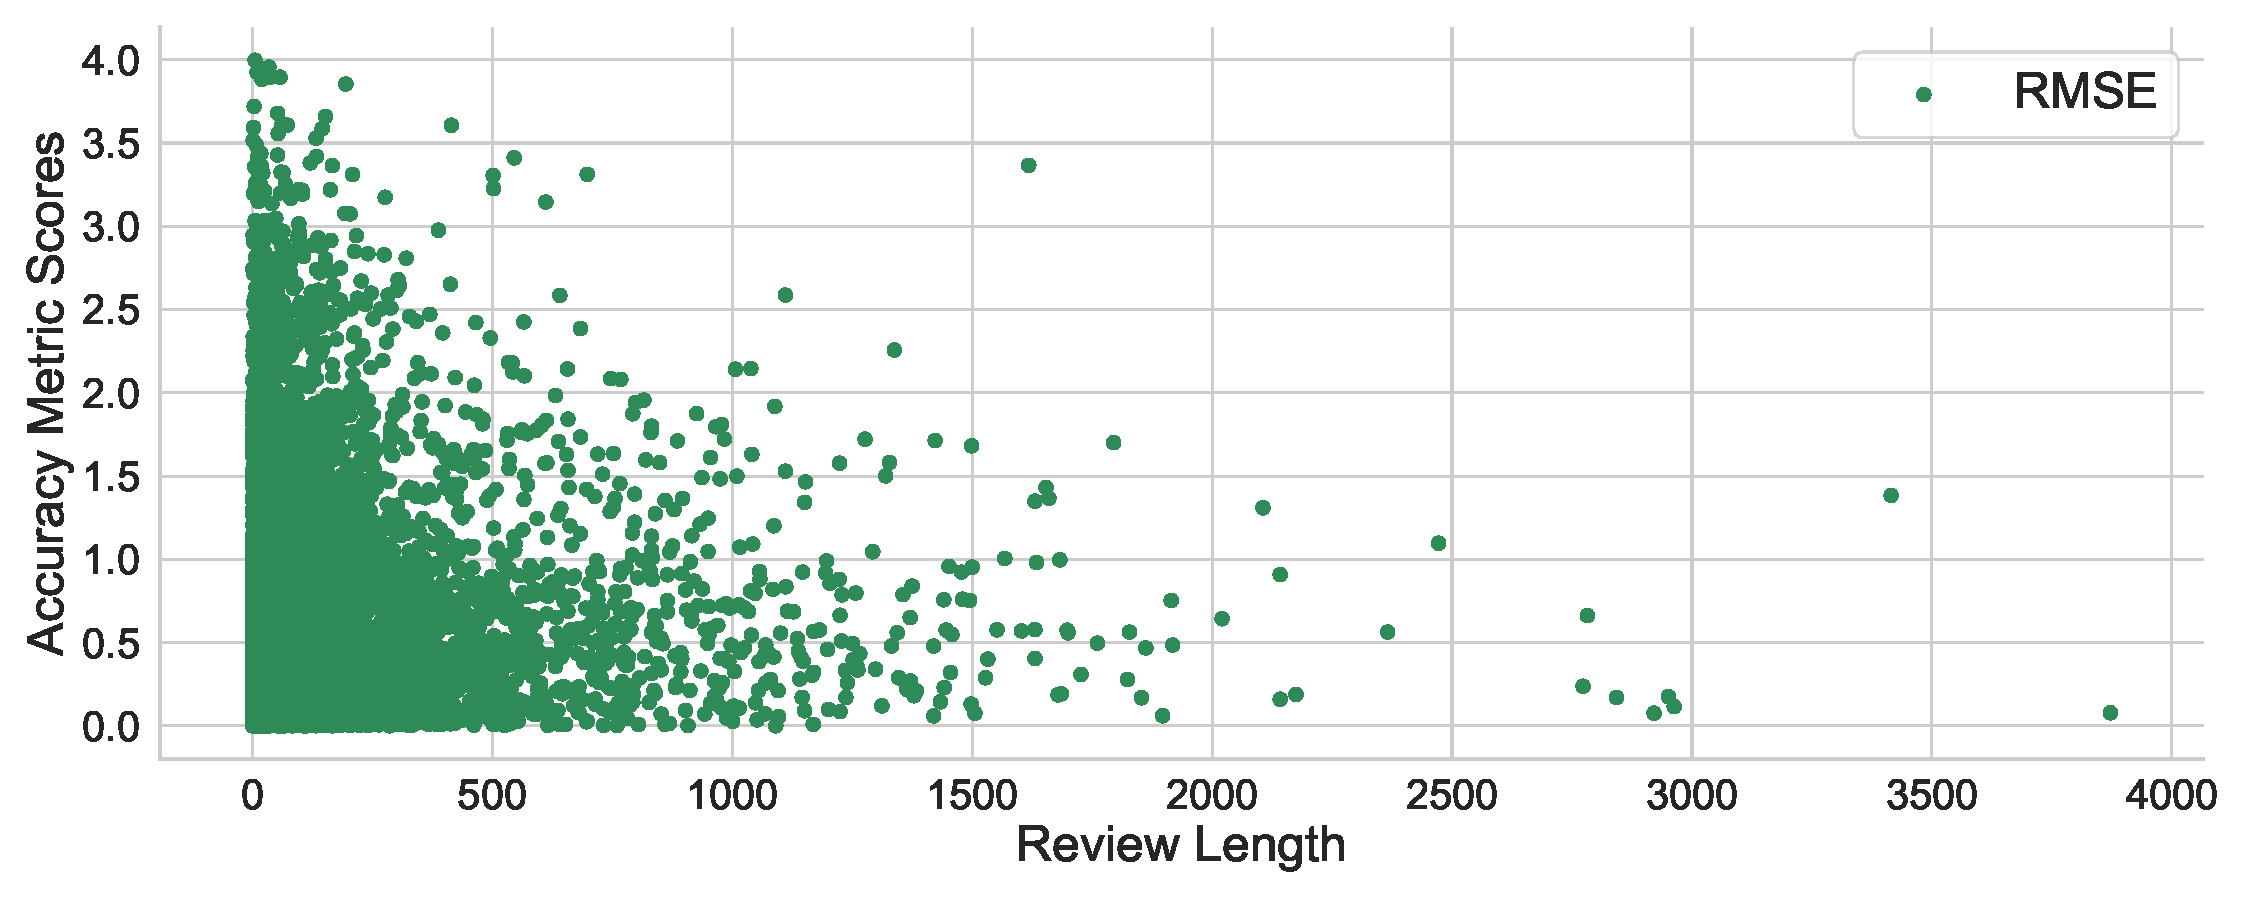
\includegraphics[width=0.99\textwidth]{Figures/ncf_length_ratings_metrics.pdf}
    \caption{RMSE against the review length in words for users.}
    \label{fig:RMSE_reviews}
\end{figure}


\begin{table}[htbp]
    \centering
    \begin{tabular}{lcccc}
        \toprule
        \textbf{Group} & \textbf{Number of Reviews}&\textbf{MAE} & \textbf{MSE} & \textbf{RMSE} \\
        \midrule
        Low & 0-6                 &             0.262 &             0.276 &              0.262 \\
        Medium & 7-31                &             0.443 &             0.585 &              0.443 \\

        High & 32-118              &             0.610   &             0.808 &              0.601   \\

        Very High & 118+                &             0.682 &             0.878 &              0.682 \\

        \bottomrule
    \end{tabular}
    \caption{Mean MAE, MSE, and RMSE for each group of users based on review length.}
    \label{tab:summary_stats_revs}
\end{table}


\subsection{Top-$N$ Results}
\label{subsec:5 Top-N Results}

As detailed in Section \ref{sec:2 Evaluation Methods}, top-$n$ recommendation represent an important aspect of recommender systems, as they reflect the system's ability to generate relevant suggestions for users \cite{lu2012recommender}. As such, this evaluation paradigm involves evaluating the effectiveness of a recommender system by considering only the top-$n$ recommendations it provides for each user. Our recommender models generated a list of $n$ items for each user. The list of $n$ items were ranked by the system's estimated rating  of each item. We can now evaluate the system's performance based on how many of the items in the top-$n$ list match with items that the user has actually interacted with or rated positively - the test set. The result of which is displayed in Table \ref{tab:top_n_res}. 

\begin{table}[htbp]
    \centering
    \begin{tabular}{|l|l|p{2cm}|l|l|l|}
    \hline
    &\textbf{Model} & \textbf{Data Used} & \textbf{Recall@100} & \textbf{Precision@100} & \textbf{F1-Score@100} \\
    \hline
    1&Item-Based Collaborative Filtering & Ratings Only & 0 & 0.0009 & 0.0001 \\
    2&User-Based Collaborative Filtering & Ratings Only & 0 & 0 & 0 \\
    3&Non-Negative Matrix Factorisation & Ratings Only & 0 & 0.0007 & 0  \\
    4&Neural Collaborative Filtering 1 & Ratings Only & 0.0007 & 0.0010 & 0.0006 \\
    5&Neural Collaborative Filtering 2 & Ratings, Reviews & 0.0007 & 0.0012 & 0.0006 \\
    6&Neural Collaborative Filtering 3 & Ratings, Reviews, Sentiments & 0.0007 & 0.0012 & 0.0006 \\
    \hline
    \end{tabular}
    \caption{Top-N Results for Recommender Models Built.}
    \label{tab:top_n_res}
\end{table}

Recall@100, Precision@100, and F1-Score@100 are metrics used to evaluate the performance of a recommender system in generating a list of top-$n$ (where $n$ is 100) recommendations for each user. As stipulated in \ref{subsec:4 Evaluation Approach}, we execute the top-$n$ evaluation for each user and then aggregate the result, to get a final mean score for each of the metrics. As mentioned, recall@100 represents the proportion of relevant items that were included in the top 100 recommendations, out of all the relevant items in the dataset \cite{cremonesi2010performance}. A higher recall@100 value indicates that the recommender system is doing a better job of capturing relevant items in its recommendations \cite{cremonesi2010performance}. In our case, all the benchmark models  have a recall@100 of 0, meaning that none of the relevant items were included in the top 100 recommendations. Similarly, for NCF models, the majority of users did not have any relevant items in their top-100 recommendations. In contrast, precision@100, which simply represents the proportion of relevant items among the top 100 recommendations \cite{cremonesi2010performance}, has scores generally above 0. The IBCF model has a precision@100 of 0.0009, which means on average, 9 out of every 100 users had 1 of their top 100 recommendations relevant, while the remaining 91 had none. The NMF model has a precision@100 of 0.0007. The NCF models had the highest precision@100 scores - NCF model with reviews (and with sentiments), achieved the highest precision score of 0.0012. Effectively, on average, 12 out of every 100 users had 1 of their top 100 recommendations relevant, while the remaining 88 had none. Finally, the F1-Score@100, which represents the harmonic mean of precision@100 and recall@100, was obtained for each model. Note, a higher F1-score@100 value indicates better overall performance in terms of capturing relevant items in the top recommendations. In our case, IBCF was the only benchmark model to have a value above 0 - F1-score@100 of 0.0001. In contrast, the NCF model's all have an F1-score@100 of 0.0006. 

\section{Discussion}
\label{sec:5 Discussion}

In this section we discuss the practical implications of the study's findings in the context of research questions. We also compare our findings with existing literature and studies in the field, highlighting areas where our results align or diverge from previous research. 

From Table \ref{tab:pred_acc_res} we identified that the family of NCF models outperformed all the other models in terms of predictive accuracy. This suggests that integrating neural networks into the collaborative framework can improve predictive accuracy. The success of NCF models can be attributed to the deep learning techniques they utilise, enabling them to learn complex relationships and patterns in the user-item interaction data \cite{he2017neural} - which they appear to achieve in this problem task.  Neural networks are capable of performing complex non-linear transformations, making them well-suited for handling the high-dimensional nature of the Amazon product review dataset. Additionally, the use of embedding layers in neural networks enables the models to capture latent features and relationships between users and items, leading to more accurate predictions \cite{he2017neural}. 

Regarding the top-$n$ evaluation, we observed that the results were less favourable.  Given the results \ref{tab:top_n_res}, our models do not appear to be doing any better than random\footnote{The probability that a random ranking correctly predicts a relevant product in the top 100 is 1-in-100.} for Top-$n$ prediction. These results can be possibly attributed to two factors. Firstly, our recommender models were primarily designed for ratings prediction rather than top-$n$ recommendations. Effectively, we adapted the models to evaluate top-$n$ recommendations, but they were not optimised for this task. Specifically, our recommender models predict ratings, so for each user we get 11 004 predicted ratings (test set). Now, suppose that only 3 products are relevant (have above the specified threshold rating, 3) for a user, on average. Our adaption of top-$n$ recommendation is then trying to see if the 3 products' ratings will come up in the top 100 of 3249. This is a tough task given that the models were not optimised for. Had the recommender models been redesigned to optimise for top-$n$ recommendations as well, we would expect the results to be very different. Several adjustments would be needed to adapt the current recommender models, such as using a different loss function like Bayesian Personalised Ranking loss, which is designed to optimise for top-$n$ recommendations \cite{rendle2010factorization}.

Secondly, the poor performance of the models in the top-$n$ evaluation may be due to the lack of diversity in the recommendations. The models may be recommending the same popular items to most users, leading to low recall and precision scores. This lack of diversity in recommendations is a common issue in collaborative filtering-based recommenders, as they tend to recommend popular items over more diverse or niche items \cite{adomavicius2005toward}. To address this issue, we can incorporate diversity measures into the recommendation process, such as item diversity or novelty, to ensure that the recommender system is recommending a variety of items to users \cite{steck2013evaluation}. This can help to improve the relevance of the recommendations and increase the chances of capturing relevant items in the top-$n$ recommendations. 

Additionally, it may be a consequence of the dataset's characteristics. From Figure \ref{fig:ratings distribution}, we identified that the ratings distribution was heavily skewed, with most ratings being 5. This skewed distribution may have impacted the system's ability to recommend diverse or niche items. When most ratings are high, it becomes challenging to differentiate between items. The heavily skewed rating distribution, in which most ratings are 5, poses a challenge to the recommender system for top-$n$ recommendations. In such cases, it becomes difficult to differentiate between good items since the predicted ratings are all close to 5. This means that the recommender system may struggle to identify items that stand out from the rest. Consequently, the system may recommend popular, mainstream items over more diverse or niche items that might also be of interest to users. To mitigate the impact of the skewed rating distribution, we can employ several strategies. We could look at incorporating implicit feedback alongside explicit ratings can provide a more comprehensive understanding of user preferences \cite{peska2017using}. Moreover, re-weighting an individual user's rating using their review text could provide a more detailed preference measure of their interest. By adjusting the original ratings, we can achieve a more accurate and reflective feedback that takes into account the nuances expressed in the reviews. This approach leverages the qualitative information provided by users, enabling a more personalised and effective recommendation system. This is another approach for incorporating review text into recommenders that has shown promising results \cite{hariri2011context}.

Ultimately, one of the foremost reasons for the poor top-$n$ results can be attributed to this analysis being focused on predictive accuracy, a task for which the models performed well, rather than for top-$n$ recommendation. Consequently, the poorer results highlighted by Table \ref{tab:top_n_res} underscore the importance of aligning the purpose of the recommender system with its evaluation criteria. This finding resonates with previous research suggesting that there is no universal best recommendation method. Instead, the success of a recommendation system is contingent upon the context and density of available data, with different methods adapting to particular applications being most likely to excel \cite{lu2012recommender}. 

\subsection{Research Questions}
\label{subsec:Research Questions}

We now revisit the research questions posed in Section \ref{sec:1 Research Questions and Significance} and discuss the implications of our findings in the context of these questions.



1. \textbf{How does incorporating product reviews into a recommender system model impact the predictive accuracy and ability to recommend relevant items?} 

The inclusion of review text enhanced the performance of the NCF model, as evidenced by a notable improvement in the MAE, MSE and RMSE for rating prediction. While the improvement in the accuracy of the predictions was significant, it is important to note that the impact on the top-$n$ evaluation was relatively smaller. 

This finding aligns with our hypothesis that leveraging review text alongside ratings data would provide a more comprehensive understanding of user preferences and lead to more accurate recommendations. The results suggest that user reviews contain valuable information that can be utilised to improve the predictive accuracy of recommender systems, especially in tasks such as rating prediction.

2. \textbf{How does incorporating review sentiment as well as review text in a recommender system impact the predictive accuracy and ability to recommend relevant items?}

The results between the NCF model with ratings, review text and review sentiments were comparable to those of the NCF model with review and ratings only. There were no substantial improvements observed with the inclusion of sentiments.

These findings suggest that the sentiment analysis technique used in this study may not have provided significant additional value in the context of the problem being addressed. However, it is important to note that this does not rule out the possibility that a more refined sentiment analysis approach could yield better results in future studies. Future work may involve exploring alternative sentiment analysis techniques or refining the existing one to further investigate the potential impact of incorporating review sentiments into recommender systems. 

In contrast to our results, several studies in the literature have found that incorporating sentiment analysis into recommender systems can improve their performance (\cite{srifi2020recommender}; \cite{roy2022systematic}). This contrast could be due to several factors, such as the specific characteristics of the Amazon product review dataset, as well as the way sentiment analysis was incorporated into the model, or even the model itself - NCF. Moreover, the choice of sentiment analysis was somewhat more sophisticated in the papers mentioned.


3. \textbf{How does the performance of the collaborative-based filtering recommender system using neural collaborative filtering compare to that of popular benchmark recommender systems?}

NCF outperformed all benchmarks for both rating prediction and top-$n$ evaluation metrics. These results signify the potential of neural architecture or deep learning introduction to enhance the accuracy and effectiveness of recommender systems. Research claims that neural networks can capture complex patterns and relationships in data, which is likely the reason for the superior performance of NCF in this study \cite{he2017neural}. Although the results for top-$n$ evaluation were less favourable, hypothesis testing confirmed that the differences in performance between NCF and the benchmark models were statistically significant. 

The superior performance of NCF over other more traditional recommender systems has been widely reported in previous literature (\cite{he2017neural}; \cite{rendle2020neural}). Similarly, other work which have used Amazon product reviews for building recommenders have found that incorporating deep learning-based approached for collaborative filtering have found improved results \cite{rezaei2021amazon}. Specifically, \cite{rezaei2021amazon} found that a deep neural network architecture for collaborative filtering outperformed traditional models in predicting review rating scores. Our findings are consistent with these studies, suggesting that neural collaborative filtering models are more effective in capturing complex user-item interactions and generating more accurate rating predictions.


4. \textbf{What are the potential trade-offs of incorporating product reviews into a recommender system, such as increased complexity or potential biases in the recommendations?}

Having implemented the solution, we acknowledge that incorporating product reviews into a recommender system introduces additional work, but not necessarily increased complexity. These reviews require additional text pre-processing which was discussed in great detail in Section \ref{subsec:3 Text Analysis and Cleaning}, and then finally require text embedding. For NCF, review text is integrated into the input layer alongside user and items.  These embeddings are then concatenated with the user and item embeddings to form the input vector for the neural network - as discussed in Section \ref{sec:4 Modelling Approach}. Within the neural network, the review text is processed alongside the user and item embeddings to generate the final rating prediction. This process is not necessarily more complex than the existing models.

To explore the computational runtimes associated with incorporating reviews compared to those models that were built without reviews, we monitored the training run times. Table \ref{tab:computational-details} provides a comparison of the run-times of various collaborative filtering models. The benchmark models show higher runtimes compared to all the NCF model instances, indicating that they may require more computational resources compared to the NCF model. This is likely due to the fact that these benchmark models were built from scratch using Python, while the NCF model was built using TensorFlow, which is optimised for deep learning tasks. Additionally, incorporating the reviews into the recommender model did increase the run time of the NCF model from 12 minutes to 13 minutes. Moreover, we note that including sentiments as well as reviews to the NCF model did not increase the computation run time compared to using reviews and ratings only. 

Overall, incorporating product reviews into a recommender system, appears to not greatly impact the runtime of the model. This is likely due to the additional complexity of incorporating reviews is not significantly higher than the existing models. Furthermore, NCF models in general, even with the additional augmented review and sentiments data run faster (13 minutes) than the quickest benchmark model - UBCF at 125 minutes. Again, this is largely due to the fact that the NCF model is built using TensorFlow, which is optimised for deep learning tasks, whilst the benchmark models were built from scratch using Python. 

\begin{table}[htbp]
    \centering
    \begin{tabular}{|l|l|l|}
    \hline
    \textbf{Model} & \textbf{Data Used} & \textbf{Runtime (minutes)} \\
    \hline
    Item-Based Collaborative Filtering & Ratings Only & 140 \\
    User-Based Collaborative Filtering & Ratings Only & 125 \\
    Non-Negative Matrix Factorisation & Ratings Only & 457 \\
    Neural Collaborative Filtering 1 & Ratings Only & 12 \\
    Neural Collaborative Filtering 2 & Ratings \& Reviews &13 \\
    Neural Collaborative Filtering 3 & Ratings, Reviews, Sentiments & 13 \\
    \hline
    \end{tabular}
    \caption{Computational Details of Various Collaborative Filtering Models}
    \label{tab:computational-details}
\end{table}

\section{Conclusion}
\label{sec:5 Conclusion for Results}

In this chapter, we presented the outcomes of our various recommender models and their implications within the context of our research questions, contrasting them with existing literature on review-aware recommenders. Effectively, this chapter is the culmination of the literature review (Chapter \ref{Chapter2}), data exploration (Chapter \ref{Chapter3}), and methodological approach (Chapter \ref{Chapter4}).

Most notably, the NCF model outperformed all the benchmark models in terms of both predictive accuracy and top-$n$ evaluation. Our findings closely align with existing research on incorporating deep learning-based techniques into the collaborative filtering network \cite{he2017neural}, where there has been some significant attention and improvements discovered. Additionally, one-sampled paired t-tests revealed that all improvements were statistically significant at a significance level of $p < 0.01$ for predictive accuracy results. Moreover, we note that the review-aware NCF model augmented with sentiments did not exhibit significant performance improvements in terms of predictive accuracy. Additionally, top-$n$ evaluation results were discussed in detail, focusing on addressing the less favourable results observed across all the recommenders. We emphasised the importance of tailoring a recommender for a specific task. Since our primary concern was predictive accuracy, our recommenders yielded  poor results in top-$n$ evaluation - often not performing better than random. Strategies for improvement were outlined, and additional factors contributing to the poor results were also addressed - namely the skew rating distribution. Effectively, this chapter highlights the importance of incorporating reviews into recommender systems, particularly through the review-aware NCF model, which provided evidence that incorporating reviews improves predictive accuracy. Although there was no substantial improvement with the inclusion of sentiments, the overall performance of the NCF model suggests promising opportunities for future exploration and optimisation. 

Importantly, we have addressed each of the four research questions posed in Section \ref{sec:1 Research Problem and Objectives}. To summarise, incorporating reviews into a recommender model does lead to an improvement in predictive accuracy. Incorporating sentiments, did not yield improved results, however there is ample opportunities for further exploration, especially in choosing more sophisticated sentiment extraction techniques. The NCF model consistently outperformed all the benchmark models, showing improvements in both predictive accuracy and top-$n$ evaluation, suggesting that the deep learning-based approach is more effective in capturing complex user-item interactions than the traditional collaborative filtering methods. Finally, incorporating reviews into a recommender system did not yield large increases in the computational complexity of the models, evidenced by the marginal increase in run times for the NCF model. 
